\documentclass{article}
\usepackage[utf8]{inputenc}
\usepackage{graphicx}
\graphicspath{ {./images/} }

\author{Mikołaj Walczak}
\title{Semantic relations in embeddings}

\begin{document}
  \maketitle
  \section{T-SNE visualization}
  \begin{figure}[ht]
    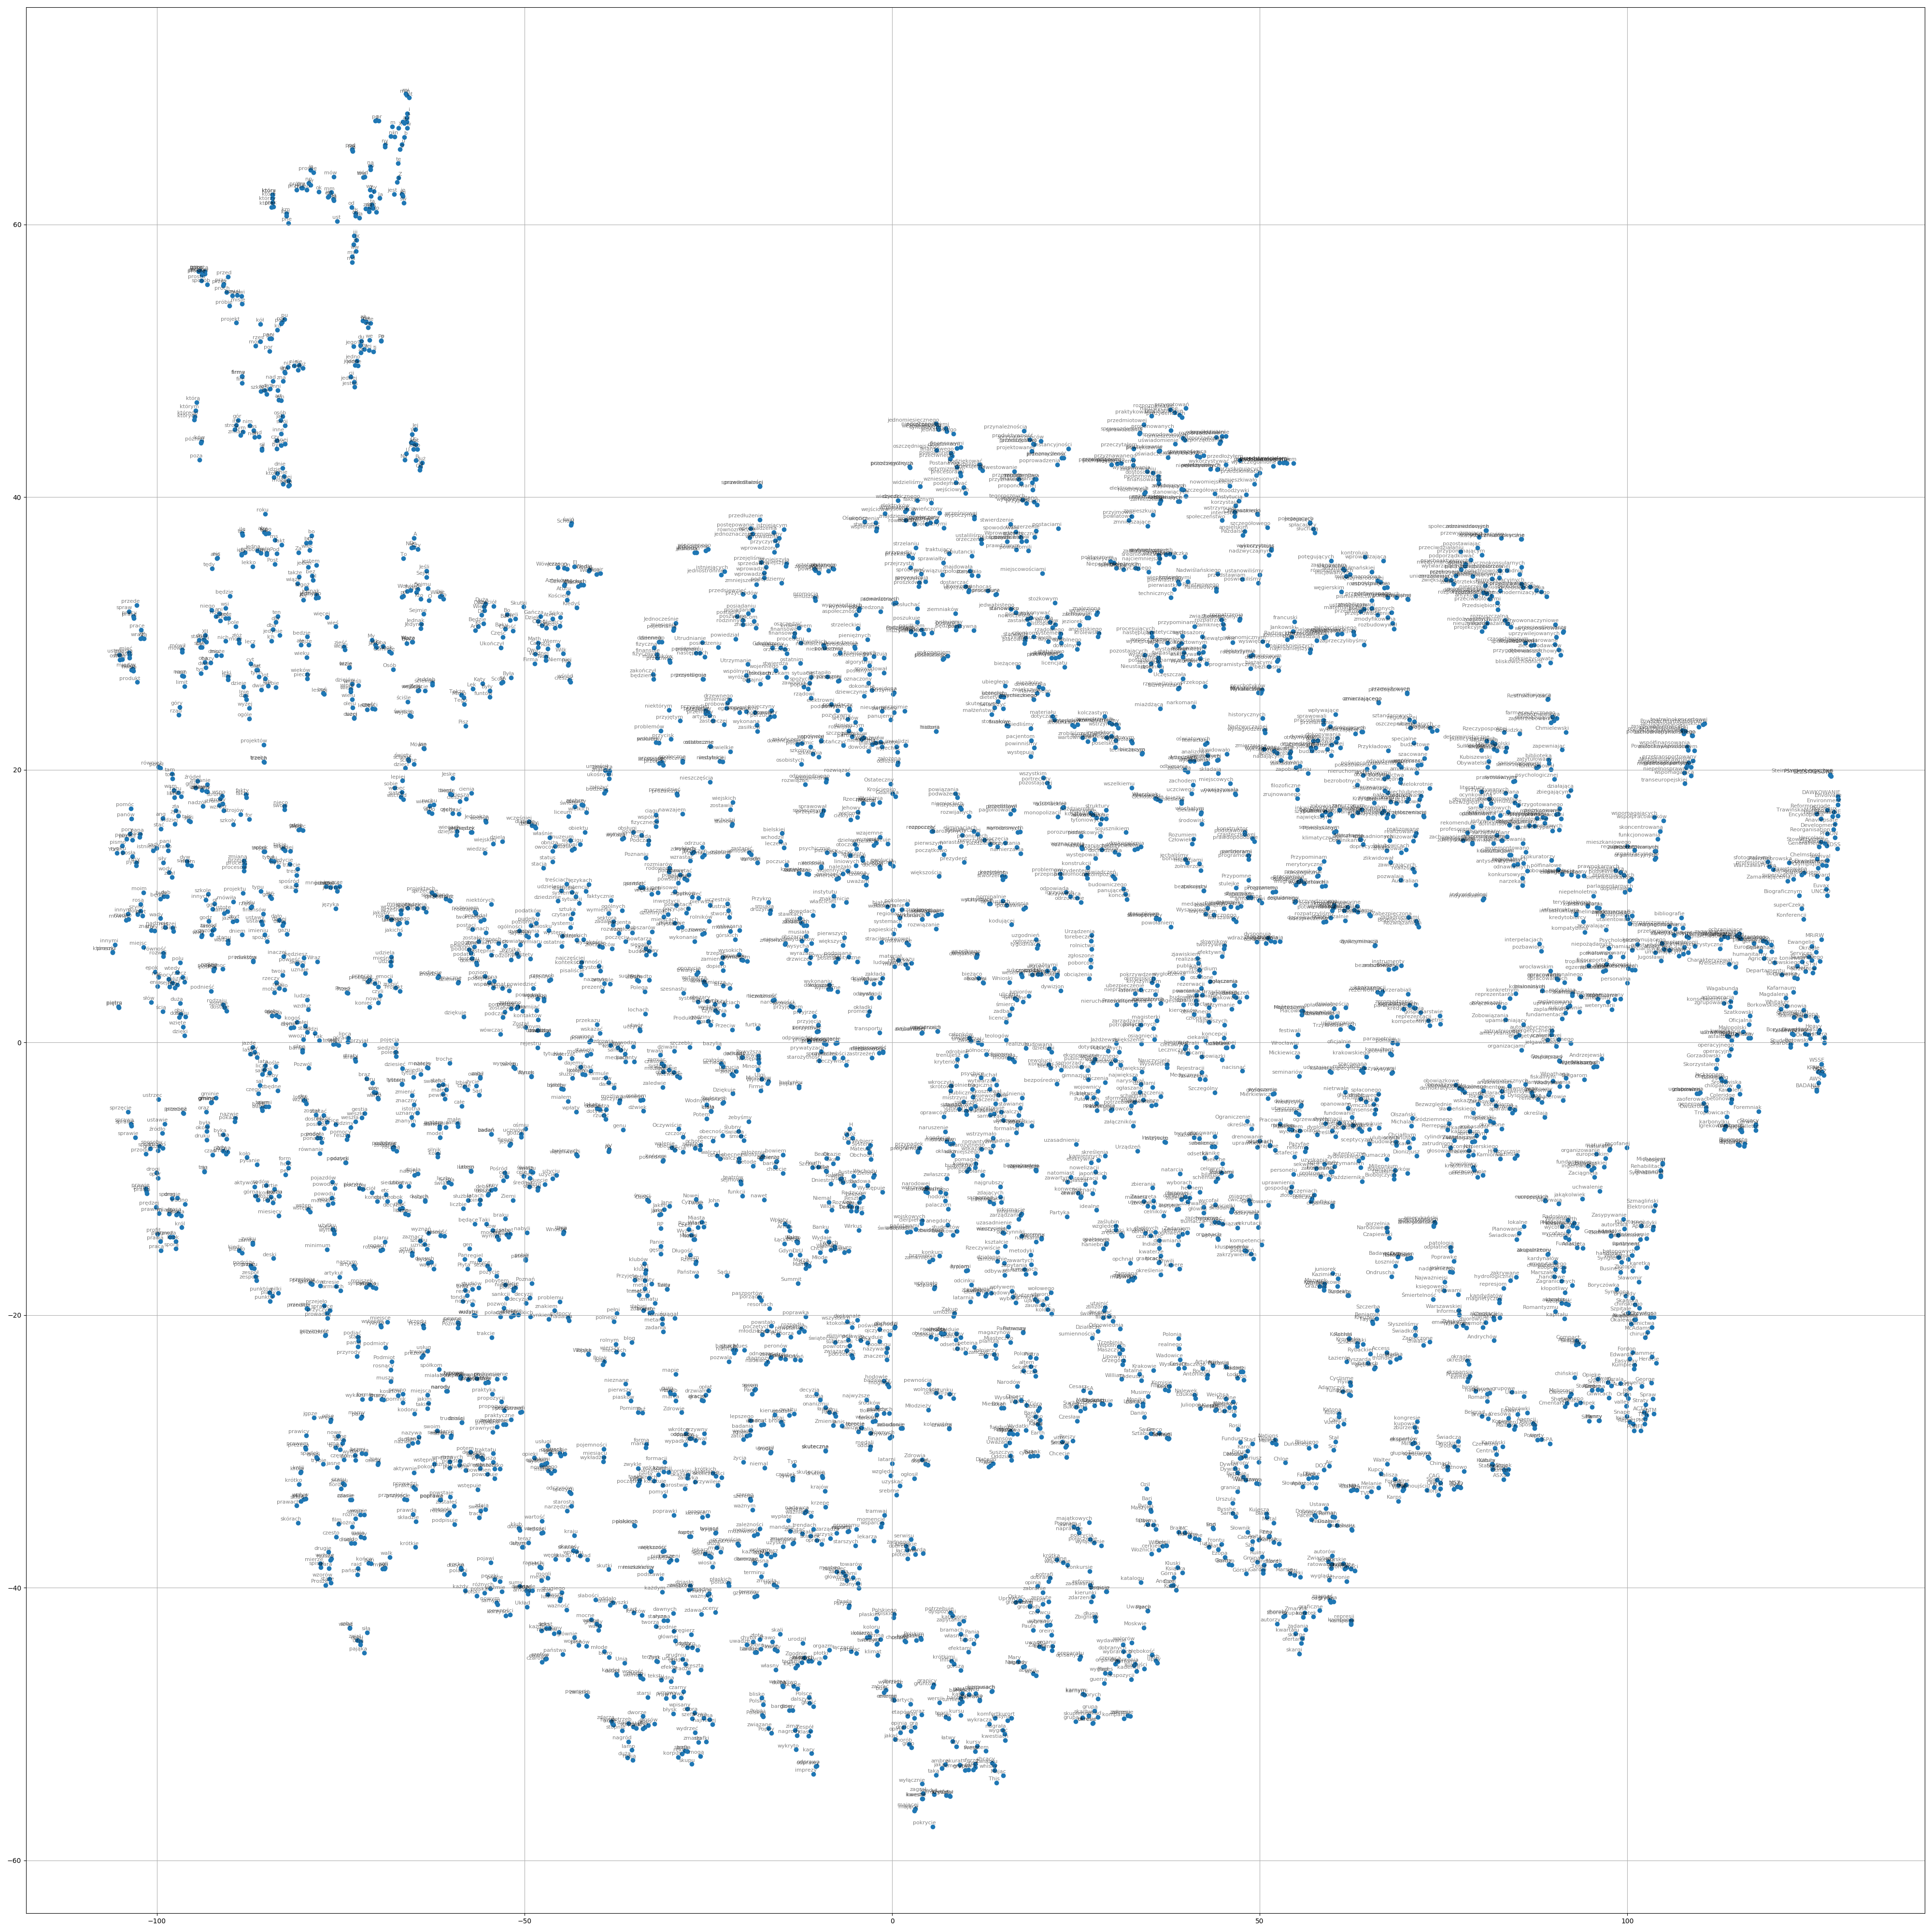
\includegraphics[width=\textwidth]{embeddings_500}
    \caption{T-SNE visualization of the first 500 words from the corpus}
    \label{fig:tsne-500}
  \end{figure}

  \section{Singular-Plural relation}
  By analizing the t-sne visualizations the most noticable relation at the first
  glance was how closely singular and plural forms of the same noun occurred on
  the graph. I have decided to analyze if we can extract a vector $\delta$ such that
  for any nouns \texttt{s} and \texttt{p} such that \texttt{p} is a plural
  form of a noun \texttt{s} the following equation holds:
  \begin{equation}
    s + \delta = p
  \end{equation}
  Where $s$ and $p$ denote embeddings for \texttt{s} and \texttt{p} accordingly.

  \subsection{Definitions}
  For convinience lets define a relation of being a plural
  \begin{equation}
    P = \{\langle s, p \rangle : \textrm{\texttt{p} is a plural of \texttt{s}} \}
  \end{equation}

  \subsection{Results}
  A set of words has been extracted to check if the relation holds. For each
  $\langle s, p \rangle \in P$ and $\langle s', p' \rangle \in P$ the cosine
  similarity has been calculated $\gamma(s' + p - s, p')$. Partial
  results can be seen in the table below (Table \ref{tab:sinpl_sim}).

  \begin{table}[ht]
  \center
    \resizebox{\textwidth}{!}{%
  \begin{tabular}{|c||c|c|c|c|c|c|}
  \hline
    & $\texttt{s}_i$/$\texttt{p}_i$ & \textit{strata/y} & \textit{miejsce/a} & \textit{umowa/y} & \textit{firma/y} & \textit{odprawa/y} \\ \hline \hline
    $\texttt{s'}_i$/$\texttt{p'}_i$ & $\delta$ & $\gamma(s_1 + \delta, p_1)$ & $\gamma(s_2 + \delta, p_2)$ & $\gamma(s_3 + \delta, p_3)$  & $\gamma(s_4 + \delta, p_4)$  & $\gamma(s_5 + \delta, p_5)$ \\ \hline
    \textit{strata/y} & $p'_1 - s'_1$ & 1 & 0.9832 & 0.9995 & 0.9969 & 0.9993 \\ \hline
    \textit{miejsce/a} & $p'_2 - s'_2$ & 0.9807 & 1 & 0.9933 & 0.9788 & 0.9983 \\ \hline
    \textit{umowa/y} & $p'_3 - s'_3$ & 0.9977 & 0.9762 & 1 & 0.9925 & 0.9991 \\ \hline
    \textit{firma/y} & $p'_4 - s'_4$ & 0.9978 & 0.9840 & 0.9988 & 1 & 0.9990 \\ \hline
    \textit{odprawa/y} & $p'_5 - s'_5$ & 0.9944 & 0.9890 & 0.9985 & 0.9878 & 1 \\ \hline
  \end{tabular}
  }
  \caption{Cosine similarity between plural and generated plural forms}
  \label{tab:sinpl_sim}
  \end{table}

  \subsection{Concerns}

  \begin{table}[ht]
  \center
    \begin{tabular}{|c|c|c|c|}
    \hline
    $i$ & $\texttt{s}_i$ & $\texttt{p}_i$ & $\gamma(s_i, p_i)$ \\ \hline
    0 & strata & straty & 0.9986 \\ \hline
    1 & miejsce & miejsca & 0.9864 \\ \hline
    2 & umowa & umowy & 0.9990 \\ \hline
    3 & firma & firmy & 0.9993 \\ \hline
    4 & odprawa & odprawy & 0.9994 \\ \hline
    \end{tabular}
  \caption{Cosine similarity between singular and plural forms}
  \label{tab:sinpl_sim_words}
  \end{table}

  For $\langle s, p \rangle \in P$ the words are syntactically similar and
  therefore close to each other, resulting in a difference vector $\delta = p - s$
  having short length. Good approximations of plural forms might be result of
  $\delta$ not affecting much the vector $s$, whcih is on its own very close to vector $p$
  (as shown in the Table \ref{tab:sinpl_sim_words}).

  Putting both tables together we can see that in most cases adding the difference
  vector puts the word further away from its plural form. Table \ref{tab:sinpl_diff}
  shows the difference $\gamma(s + \delta, p) - \gamma(s, p)$ for each $\delta = p' - s'$
  where $\langle s', p' \rangle \in P$.

  \begin{table}[ht]
  \center
    \resizebox{\textwidth}{!}{%
  \begin{tabular}{|c||c||c|c|c|c|c|}
  \hline
     & $\delta$ & $\gamma(s_1 + \delta, p_1)$ & $\gamma(s_2 + \delta, p_2)$ & $\gamma(s_3 + \delta, p_3)$  & $\gamma(s_4 + \delta, p_4)$  & $\gamma(s_5 + \delta, p_5)$ \\ \hline \hline
    $\gamma(s_1, p_1)$ & $p_1 - s_1$ & 0.0013 & -0.015 & 0.0009 & -0.001 & 0.0006 \\ \hline
    $\gamma(s_2, p_2)$ & $p_2 - s_2$ & -0.005 & 0.0135 & 0.0068 & -0.007 & 0.0118 \\ \hline
    $\gamma(s_3, p_3)$ & $p_3 - s_3$ & -0.001 & -0.022 & 0.0010 & -0.006 & 0.0009 \\ \hline
    $\gamma(s_4, p_4)$ & $p_4 - s_4$ & -0.001 & -0.015 & -0.004 & 0.0007 & -0.002 \\ \hline
    $\gamma(s_5, p_5)$ & $p_5 - s_5$ & -0.005 & -0.010 & -0.001 & -0.011 & 0.0006 \\ \hline
  \end{tabular}
  }
  \caption{Cosine similarity between plural and generated plural forms}
  \label{tab:sinpl_diff}
  \end{table}

  \section{Foreign Names cluster}
  Foreign names seem to form a cluster, calculating cosine similarity between
  all of the pairs confirm the prediction made based on the visualization.

  \begin{table}[ht]
  \center
    \begin{tabular}{|c|c|c|c|c|c|c|}
    \hline
     & George & Severus & Orton & Snape & Edwarda & Fordon \\ \hline
    George & 1.0000 & 0.9967 & 0.9971 & 0.9950 & 0.9964 & 0.9969 \\ \hline
    Severus & 0.9967 & 1.0000 & 0.9972 & 0.9950 & 0.9940 & 0.9946 \\ \hline
    Orton & 0.9971 & 0.9972 & 1.0000 & 0.9982 & 0.9957 & 0.9965 \\ \hline
    Snape & 0.9950 & 0.9950 & 0.9982 & 1.0000 & 0.9962 & 0.9951 \\ \hline
    Edwarda & 0.9964 & 0.9940 & 0.9957 & 0.9962 & 1.0000 & 0.9989 \\ \hline
    Fordon & 0.9969 & 0.9946 & 0.9965 & 0.9951 & 0.9989 & 1.0000 \\ \hline
    \end{tabular}
  \caption{Cosine similarity of foreign names}
  \label{tab:foreign_names}
  \end{table}
\end{document}
